\subsection{DATOS}
Amplificador Operacional LM324.

$Vcc = 10V$  $Vss = -10V$

$R1 = R2 = R3 = R4 = R5 = R$

\begin{center}
	\resizebox{14cm}{!}{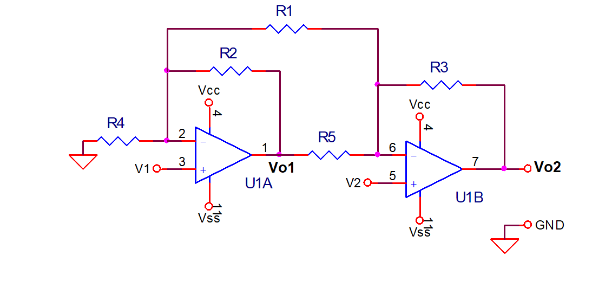
\includegraphics{Imagenes/CI.png}} \\
	\stepcounter{figure}
	\begin{center}
    	\begin{small}
        \textit{Fig.\thefigure \ - \ 	Circuito I: Amplificador Diferencial.}
		\end{small}
    \end{center}
\end{center}

\subsection{PARÁMETROS/RELACIONES A ANALIZAR:}

\noindent \textbf{ANALÍTICO:} $(V_{C}= ( V_{1} + V_{2} )/2$ \space $V_{D} =( V_{2} - V_{1} ) )$
\begin{enumerate}[\one .1]
    \item $V_{o1} = f(V_{1}, V_{2} )$; $V_{o1} = f(V_{D} ,V_{C} )$
    \item $V_{o2} = f(V_{1}, V_{2} )$; $V_{o2} = f(V_{D} ,V_{C} )$
    \item Impedancia vista por las fuentes de señal.
\end{enumerate}

\subsection{MEDICIÓN - SIMULACIÓN:}
\begin{enumerate}[\one.4]
    \item[\one.4] {Gráfico Entrada/Salida: $V_{o1}=f(V_{1})$\hspace{0.25cm} y \hspace{0.25cm} $V_{o1} = f(V_{2})$ \hspace{0.25cm}$Vss < V_{1}$\hspace{0.25cm} , $V_{2} < Vcc$}
    
    \item[\one.5] {Gráfico Entrada/Salida: $V_{o1}=f(V_{C} )$\hspace{0.25cm} y \hspace{0.25cm}$V_{o2} = f(V_{C} )$\hspace{0.25cm} $Vss<V_{C}< Vcc$}
\end{enumerate}
